%% Based on  LaTeX template for MLP 2018, modified from ICML 2017 - example_paper.tex at 
%%  https://2017.icml.cc/Conferences/2017/StyleAuthorInstructions

\documentclass[11pt]{article}
\usepackage[T1]{fontenc}
\usepackage{amssymb,amsmath}
\usepackage{txfonts}
\usepackage{microtype}
\usepackage{xspace}
\xspaceaddexceptions{\%}

% Lists with less spacoing between items
\usepackage{paralist}

% For figures
\usepackage{graphicx}
\usepackage{subfig} 


% For algorithms
\usepackage{algorithm}
\usepackage{algorithmic}

% the hyperref package is used to produce hyperlinks in the
% resulting PDF.  If this breaks your system, please commend out the
% following usepackage line and replace \usepackage{mlp2017} with
% \usepackage[nohyperref]{mlp2017} below.
\usepackage{hyperref}
\usepackage{url}
\urlstyle{same}

% Packages hyperref and algorithmic misbehave sometimes.  We can fix
% this with the following command.
\newcommand{\theHalgorithm}{\arabic{algorithm}}


% Set up MLP coursework style (based on ICML style)
\usepackage{style}
\bibliographystyle{ieeetr}
\mytitlerunning{Msc Project Progress Report}

\DeclareMathOperator{\softmax}{softmax}
\DeclareMathOperator{\sigmoid}{sigmoid}
\DeclareMathOperator{\sgn}{sgn}
\DeclareMathOperator{\relu}{relu}
\DeclareMathOperator{\lrelu}{lrelu}
\DeclareMathOperator{\elu}{elu}
\DeclareMathOperator{\selu}{selu}
\DeclareMathOperator{\maxout}{maxout}






\usepackage{cprotect}
\usepackage{subfig}
\usepackage{enumitem}

\def\studentNumber{s1843212}

\begin{document} 


\mytitle{Msc Project Progress Report: Developing an\\Application to
Introduce Parallel Task Scheduling}
\centerline{\studentNumber}
\vskip 7mm


\section{Goal of Project}

The goal of this project is to develop an game like application to introduce parallel task scheduling to students and to help the students to learn. The content should cover a variety of concepts in this area. For example:

\begin{itemize}
    \item What is task graph in parallel computing and how it's related to real world problems.
    \item What are clusters and varieties of clusters when analyzing task scheduling problems.
    \item General problems in this area like communication cost and heterogeneous clusters.
    \item General techniques in this area for performance improvements like keeping tasks on same processor to minimize communication cost.
    \item Common algorithms for task graph scheduling and their applicable type of cluster.
\end{itemize}

\section{Methods Used}

This project focuses on development of the application. The current technical choice is LWJGL on Java, which includes Java binding of OpenGL, OpenAL and several other native libraries, same as described in project proposal. It is chosen because it provides cross platform support for hardware rendering, which enables better performance and produces more flexibility in development like manual matrix control and immediate rendering. The drawback of the choice is that work is required to implement an abstract layer over low level APIs to build a complex application.

This application uses many levels (or missions) to introduce different aspects of the concept. Some may ask the student to simulate the behavior of standard algorithms, while some may ask the student to provide the schedule that finishes within a period of time, with the help of specific techniques. It encourages students to do experiments and shows the result, to provide an intuitive learning experience and to reinforces the understanding.

\section{Current State}

\begin{figure*}[t]
    \centering
    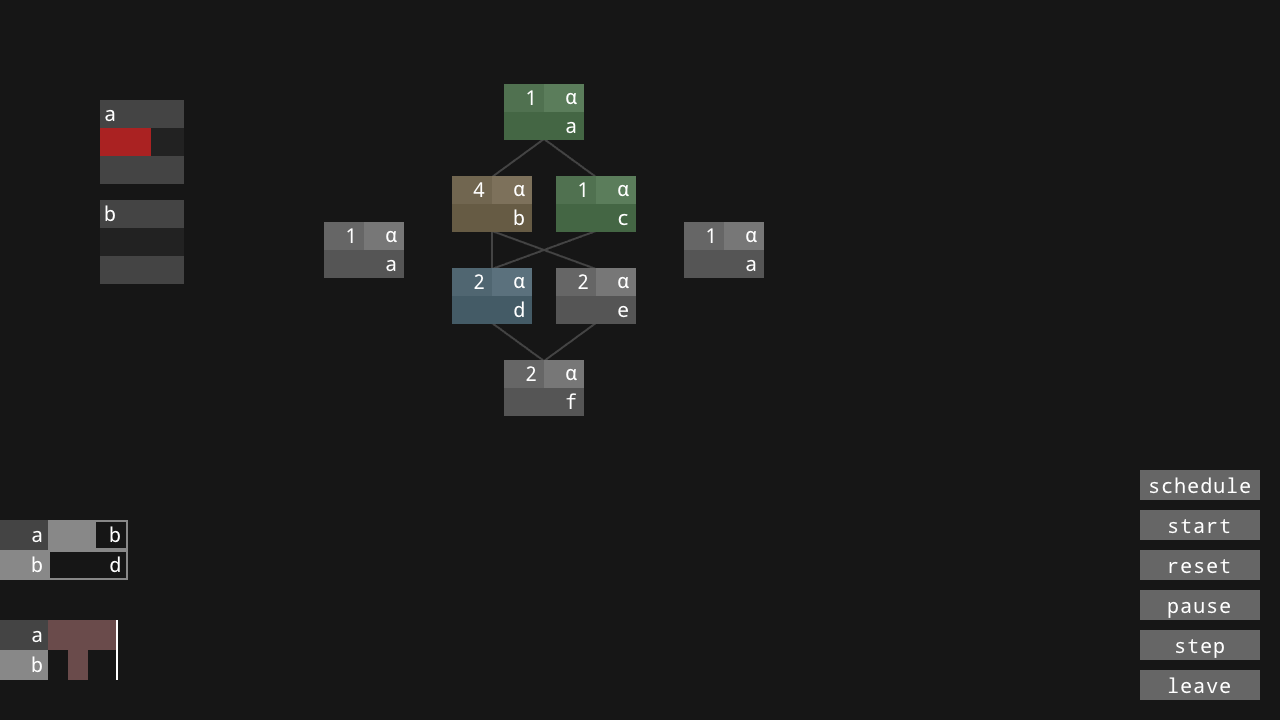
\includegraphics[width=\textwidth]{screenshot.png}
    \caption{Screenshot of the application. The upper left shows the state of processors. The upper right shows three task graphs. The bottom shows task queues and execution timeline. Every task has three elements: duration, type and name. In a task graph, a task is grey when unassigned, blue when assigned, yellow when processing and green when finished.}
    \label{fig}
\end{figure*}

Figure \ref{fig} shows a screenshot of the application. Inside the interface, the user can drag tasks to assign them into queues of each processor and the engine will execute them automatically and display the history of each processor. Although the interface is still missing some details, it seems many parts are working correctly. Up to now, this project contains over 5k lines of code and the components listed below has been finished:

\begin{itemize}
    \item A flexible GUI framework using immediate rendering based on OpenGL.
    \item Many widgets with advanced features like drag and drop, animation and cursor highlight.
    \item A simple sound system based on OpenAL.
    \item An engine to simulate execution of task graph on clusters with different configurations.
    \item Data driven models for games, graphs and clusters to program levels.
    \item A algorithm systems to let the user develop and run customized algorithms. 
\end{itemize}

\section{Future Plan}

In the remaining time, two things will be done. The first is to implement the tutorial system to introduce the mechanisms of the system and standard algorithms. It requires some tweaks to the GUI framework and much text writing. So it could take some time to finish. Another thing is user testing. One week will be reserved for it.

If time allows, extra features will be added to the application, like multiplayer mode and testing mode. Decisions will be made according to 
progress. Also, extra details will be added to the interface to make it more appealing.

\end{document} 
